\documentclass[a4paper]{report}
\usepackage[utf8]{inputenc}
\usepackage[T1]{fontenc}
\usepackage{RJournal}
\usepackage{amsmath,amssymb,array}
\usepackage{booktabs}


% tightlist command for lists without linebreak
\providecommand{\tightlist}{%
  \setlength{\itemsep}{0pt}\setlength{\parskip}{0pt}}

\usepackage{longtable}

% Always define CSL refs as bib entries are contained in separate doc
% Pandoc citation processing
\newlength{\cslhangindent}
\setlength{\cslhangindent}{1.5em}
\newlength{\csllabelwidth}
\setlength{\csllabelwidth}{3em}
\newlength{\cslentryspacingunit} % times entry-spacing
\setlength{\cslentryspacingunit}{\parskip}
% for Pandoc 2.8 to 2.10.1
\newenvironment{cslreferences}%
  {}%
  {\par}
% For Pandoc 2.11+
\newenvironment{CSLReferences}[2] % #1 hanging-ident, #2 entry spacing
 {% don't indent paragraphs
  \setlength{\parindent}{0pt}
  % turn on hanging indent if param 1 is 1
  \ifodd #1
  \let\oldpar\par
  \def\par{\hangindent=\cslhangindent\oldpar}
  \fi
  % set entry spacing
  \setlength{\parskip}{#2\cslentryspacingunit}
 }%
 {}
\usepackage{calc}
\newcommand{\CSLBlock}[1]{#1\hfill\break}
\newcommand{\CSLLeftMargin}[1]{\parbox[t]{\csllabelwidth}{#1}}
\newcommand{\CSLRightInline}[1]{\parbox[t]{\linewidth - \csllabelwidth}{#1}\break}
\newcommand{\CSLIndent}[1]{\hspace{\cslhangindent}#1}



\begin{document}


%% do not edit, for illustration only
\sectionhead{Contributed research article}
\volume{16}
\volnumber{4}
\year{2024}
\month{December}
\setcounter{page}{102}

\begin{article}
  % !TeX root = RJwrapper.tex
\title{Calculating Standardised Indices Using SEI}


\author{by Sam Allen and Noelia Otero}

\maketitle

\abstract{%
Standardised indices are measurements of variables on a standardised scale. The standardised scale facilitates comparisons between different variables, and its probabilistic interpretation means the indices are effective for risk management and decision making. Standardised indices have become popular in weather and climate settings, for example within operational drought monitoring systems, and have also been applied in other contexts, such as to energy variables. To facilitate their implementation in practice, the SEI package in R allows the flexible calculation of standardised indices. This paper discusses the theory underlying well-known standardised indices, outlines the general framework to construct them, and provides implementation details for the SEI package. Two case studies are presented whereby standardised indices are applied to climate and energy variables.
}

\hypertarget{introduction}{%
\section{Introduction}\label{introduction}}

Monitoring the values of a variable over time allows practitioners to not only identify long term patterns in the variables of interest, but also to analyse abnormal situations with potentially adverse socio-economic consequences. However, it can be difficult to compare time series of variables defined on different scales. For example, different spatial regions have different climates, meaning a rainfall event that is impactful at one location may not be at another. Similarly, energy demand will depend on the local climate, as well as on installed energy capacities. To account for this, it is convenient to transform variables onto the same, standardised scale. The resulting standardised variables are often referred to as \emph{standardised indices}.

Well-known examples of standardised indices include the Standardised Precipitation Index (SPI) \citep{MckeeEtAl1993} and Standardised Precipitation Evapotranspiration Index (SPEI) \citep{VicenteEtAl2010}, which are ubiquitously used to monitor hydrometeorological droughts \citep{BegueriaEtAl2014}. The framework used to construct the SPI and SPEI is simple and interpretable, framing the observed values in terms of their similarity to past values. As such, while other methods of standardisation exist, this framework has also been used to construct many other weather and climate indices.

This includes, for example, a Standardised Runoff Index \citep{ShuklaWood2008}, a Standardised Streamflow Index \citep{VicenteEtAl2012}, a Standardised Groundwater Index \citep{BloomfieldMarchant2013}, and a Standardised Temperature Index \citep{ZscheischlerEtAl2014}. Multivariate extensions of these standardised indices have also been proposed \citep{ErhardtCzado2018}. \cite{HaoEtAl2019}, for example, define a Standardised Compound Event Index, which is used by \cite{LiEtAl2021} to construct a Standardised Compound Drought and Heat Index. Outside of a weather and climate context, \cite{AllenOtero2023} introduced analogues of the SPI and SPEI that can be used to monitor energy supply and demand. This general framework for constructing standardised indices can be applied to any variable of interest, not just those previously considered in the literature.

There are several benefits to these standardised indices. The indices are easy to interpret, and are defined on a scale with a probabilistic interpretation, making them useful tools for risk management and decision making. Standardised indices therefore provide an appealing framework with which to define shortages, or droughts, in the variable of interest. Since the standardisation can be performed separately in different conditions, for example in different seasons and locations, these shortages can be defined in a relative sense, allowing their intensity in the different conditions to be compared. As summarised by \cite{ZargarEtAl2011}, standardised indices provide a ``pragmatic way to assimilate large amounts of data into a quantitative information that can be used in applications such as drought forecasting, declaring
drought levels, contingency planning and impact assessment.''

As a result, several software packages have been developed to apply standardised indices in practice. The \CRANpkg{SCI} package \citep{SCI} in the programming language R provides the functionality to calculate several standardised climate indices. The \CRANpkg{SPEI} package \citep{SPEI-R}, also in R, contains more comprehensive functionality for the SPI and SPEI, and the \pkg{standard-precip} package \citep{standard-precip} has transferred this functionality to the programming language Python \citep{Python}. The \pkg{spei} package \citep{spei-python} in Python additionally allows computation of the SPI and SPEI, as well as the Standardised Runoff and Groundwater Indices, while the \pkg{climate-indices} package in Python also provides functionality to compute the SPI, SPEI, and other drought indices. The developmental package \pkg{standaRdized} \citep{standaRdized} can also be used for this purpose, while the \CRANpkg{SPIGA} package \citep{SPIGA} in R allows the SPI to be calculated using genetic algorithms.

However, existing software packages are limited in their flexibility, with functionality typically restricted to particular standardised indices (generally the SPI and SPEI), and particular assumptions about the reference data or parametric distributions used to calculate the indices (see next section for details). In this paper, we introduce the \CRANpkg{SEI} R package, which seeks to assimilate the advantages of these various packages to provide a flexible and comprehensive software package with which to calculate standardised indices. In particular, the package is not designed solely for climate indices, and is therefore applicable in much broader generality. The package can handle variables defined on any time scale and with any (possibly non-stationary) underlying distribution, permits user-specified reference data when calculating the indices, and additionally provides plot capabilities to visualise the resulting standardised indices.

The following section provides theoretical background on standardised indices and describes the general formula to construct them. Section 3 discusses diagnostic checks that confirm the standardisation was appropriate, while Section 4 demonstrates how the \CRANpkg{SEI} package can be used to calculate standardised indices in practice. Two applications are then presented in Section 5, whereby the \CRANpkg{SEI} package is used to calculate standardised energy indices based on time series of renewable energy production, as well as standardised wind speed indices. Section 6 concludes the paper and discusses possible extensions to the package.

\hypertarget{how-to-construct-standardised-indices}{%
\section{How to construct standardised indices}\label{how-to-construct-standardised-indices}}

There is no unique way to define standardised indices. However, several widely-adopted indices are constructed using the same, simple procedure. Using this procedure, standardised indices are straightforward to calculate, can be defined on any timescale, and behave in a relative sense, meaning they can readily be compared for different variables, spatial regions, or points in time.

The general approach is to choose a univariate variable \(X\) that measures the quantity of interest, and then to estimate \(X\)'s distribution: in the SPI, \(X\) represents the precipitation accumulation aggregated over the time scale of interest, which is usually assumed to follow a gamma distribution; in the SPEI, \(X\) represents the difference between precipitation and evapotranspiration, which is usually assumed to follow a log-logistic distribution; in the standardised temperature index, \(X\) represents the temperature, which is usually assumed to follow a normal distribution. More complicated variables have also been considered. \cite{HaoEtAl2019}, for example, consider \(X\) to be the probability of a simultaneously hot and dry event, as derived from a copula analysis.

The distribution of \(X\) is typically estimated from an archive of realisations, \(x_{1}, \dots, x_{n}\). These could represent precipitation accumulations in different months, for example, or energy demand on different days. It is common to make parametric assumptions about the distribution, as in the examples above, though non- and semi-parametric density estimation methods could also be employed. The choice of distribution is discussed in detail in the following section. In any case, the distributional assumptions must be verified when the index is calculated.

Let \(F\) denote the distribution function of \(X\), and let \(\hat{F}\) denote an estimate of \(F\) obtained from \(x_{1}, \dots, x_{n}\). If \(F\) is continuous, then the \emph{probability integral transform} (PIT) \(F(X)\) will be standard uniformly distributed. Hence, this transformation provides a convenient approach with which to standardise a (possibly new) random observation \(X^{*}\) (with realisation denoted \(x^{*}\)): the PIT value \(\hat{F}(x^{*})\) denotes the relative position of the observation \(x^{*}\) within the distribution \(\hat{F}\). If \(x^{*}\) is large relative to \(\hat{F}\), then the PIT value will be close to one; if \(x^{*}\) is small relative to \(\hat{F}\), then the PIT value will be close to zero.

This \emph{PIT variable} \(\hat{F}(X^{*})\) is bounded between 0 and 1, with values intrinsically linked to probabilities. This therefore itself provides a standardised index of sorts. This PIT variable can also be rescaled using \(2\hat{F}(X^{*}) - 1\) to get an index that is centred at zero and bounded between -1 and 1, though it is more common to use the Gaussian quantile function \(\Phi^{-1}\) to transform \(\hat{F}(X^{*})\). In this case, if \(X^{*}\) is identically distributed to \(X\), and \(\hat{F}\) is a good approximation of \(F\), then the standardised index will follow a standard normal distribution.

That is, for any variable of interest, the probability integral transform can be used to define three different types of standardised indices:

\begin{itemize}
\tightlist
\item
  \emph{Normal indices}: \(\Phi^{-1}(\hat{F}(X^{*}))\)
\item
  \emph{Probability indices}: \(\hat{F}(X^{*})\)
\item
  \emph{Bounded indices}: \(2\hat{F}(X^{*}) - 1\)
\end{itemize}

All three types of indices can be calculated from observations of the variable \(X\) and an estimate of its distribution \(F\). Since they are defined as increasing functions of PIT values, these standardised indices all quantify the relative position of an observation \(x^{*}\) within the previously observed sample \(x_{1}, \dots, x_{n}\), making them easy to interpret.

In practice, it is most common to use normal indices, though one could argue that probability and bounded indices have a more direct probabilistic interpretation. For example, if we observe the 90\(^{th}\) percentile of \(X\), then (assuming \(F\) is correctly estimated) the corresponding normal index will be 1.28, the 90\(^{th}\) percentile of the standard normal distribution, whereas the probability index will be 0.9, and the bounded index will be 0.8. Similarly, for the 10\(^{th}\) percentile of \(X\), the normal index will be -1.28, the probability index will be 0.1, and the bounded index will be -0.8. For the median of \(X\), the normal and bounded indices will be zero, whereas the probability index will be 0.5.

The general framework can therefore be summarised as follows.

\begin{itemize}
\tightlist
\item
  Estimate \(F\) from the observations \(x_{1}, \dots, x_{n}\).
\item
  Check that the estimate \(\hat{F}\) correctly fits the data.
\item
  Apply \(\hat{F}\) to an observation \(x^{*}\) (or several observations).
\item
  Transform \(\hat{F}(x^{*})\) so that the index is on the desired scale.
\end{itemize}

The probabilistic interpretation of these standardised indices has made them a useful tool when analysing shortages and excesses of the variable \(X\). This was first proposed by \cite{MckeeEtAl1993} in the context of hydrometeorological droughts, and \cite{AllenOtero2023} demonstrate that the same framework can be employed to define droughts in energy systems. In this case, droughts are defined when the standardised index exceeds or falls below a relevant threshold. Different classes of droughts can be defined using different thresholds, with a more severe drought corresponding to a more extreme threshold.

Following \cite{MckeeEtAl1993}, it is most common to study three categories of droughts, typically labelled ``Moderate'', ``Severe'', and ``Extreme'' droughts. These often correspond to the thresholds 1, 1.5, and 2 of the normal standardised indices, respectively, though the thresholds 1.28, 1.64, and 1.96 are also often used, which correspond to quantiles of the standard normal distribution. This assumes that a drought is defined as an exceedance of a threshold, though the negative of these values could analogously be used when interest is on values that fall below a threshold. Table 1 gives corresponding threshold values for the other two types of indices.

\begin{longtable}[]{@{}ccccccc@{}}
\caption{\label{tab:unnamed-chunk-1}Possible thresholds used to define droughts when using each of the three types of standardised indices. Values are shown for droughts defined when the index falls below (left) and exceeds (right) the threshold.}\tabularnewline
\toprule\noalign{}
Index Type & Extreme & Severe & Moderate & Moderate & Severe & Extreme \\
\midrule\noalign{}
\endfirsthead
\toprule\noalign{}
Index Type & Extreme & Severe & Moderate & Moderate & Severe & Extreme \\
\midrule\noalign{}
\endhead
\bottomrule\noalign{}
\endlastfoot
Normal (\texttt{normal}) & -1.96 & -1.64 & -1.28 & 1.28 & 1.64 & 1.96 \\
Probability (\texttt{prob01}) & 0.025 & 0.05 & 0.1 & 0.9 & 0.95 & 0.975 \\
Bounded (\texttt{prob11}) & -0.95 & -0.9 & -0.9 & 0.8 & 0.9 & 0.95 \\
\end{longtable}

The \CRANpkg{SEI} package allows the computation of all three types of indices, and additionally allows drought occurrences and characteristics to be computed from a time series of standardised indices.

\hypertarget{the-choice-of-distribution}{%
\section{The choice of distribution}\label{the-choice-of-distribution}}

\hypertarget{stationary-distribution-estimation}{%
\subsection{Stationary distribution estimation}\label{stationary-distribution-estimation}}

The construction of standardised indices relies on an estimate of the distribution function \(F\). This has led to much debate about what distributional assumptions are most appropriate. Consider the SPI, for example. \cite{MckeeEtAl1993} initially introduced the SPI using the gamma distribution to model \(F\). However, \cite{Guttman1999} argued that the Pearson III distribution is more appropriate, due to the additional flexibility afforded by an extra parameter, while results in \cite{StaggeEtAl2015} suggest the Weibull distribution fits the monthly precipitation accumulations in their study better than alternative parametric choices. \cite{RussoEtAl2013} also consider using non-stationary distributions that include parameters that depend on time, while \cite{LiEtAl2015} incorporate additional covariates based on other climate variables. In reality, there is generally no true parametric distribution underlying the data, and the optimal assumptions will change depending on the data under consideration.

As an alternative, it has been argued \citep[e.g.][]{ErhardtCzado2018,HaoEtAl2019,AllenOtero2023} that the choice of a parametric distribution can be circumvented by using the empirical distribution function of the observations,

\begin{equation}
\hat{F}_{n}(x) = \frac{1}{n} \sum_{i=1}^{n} 1 \{ x_{i} \leq x \},
\end{equation}

where \(1\{ \cdot \}\) is equal to one if the statement inside the brackets is true, and zero otherwise. It is common to rescale \(\hat{F}_{n}(x)\) so that it is never equal to zero or one, thereby ensuring that the (normal) standardised indices are real-valued; for example, using \((n \hat{F}_{n}(x) + 1)/(n + 2)\). The empirical distribution function returns a standardised index that can only take on \(n + 1\) possible values. This is not an issue in practice if \(n\) is large, but can become problematic with smaller sample sizes, particularly when interest is on extreme events.

\cite{AllenOtero2023} propose the use of semi-parametric density estimation methods, which provide a compromise between parsimonious parametric distributions and the empirical distribution function. For example, kernel density estimators estimate the density function \(f\) corresponding to \(F\) using
\[
\hat{f}(x) = \frac{1}{nh} \sum_{i=1}^{n} K \left( \frac{x - x_{i}}{h} \right),
\]
where \(K\) is a kernel function, and \(h > 0\) is a smoothing parameter called the bandwidth. The \CRANpkg{SEI} package provides functionality to perform kernel density estimation using a Gaussian kernel. Non- and semi-parametric density estimation methods are considerably more flexible than parametric methods, though they require more data to accurately model \(F\). Further details about density estimation methods can be found, for example, in \cite{Silverman2018}.

\begin{longtable}[]{@{}ccc@{}}
\caption{\label{tab:unnamed-chunk-2}Distributions available in \CRANpkg{SEI}, and their supports.}\tabularnewline
\toprule\noalign{}
Distribution & Argument Code & Support \\
\midrule\noalign{}
\endfirsthead
\toprule\noalign{}
Distribution & Argument Code & Support \\
\midrule\noalign{}
\endhead
\bottomrule\noalign{}
\endlastfoot
Empirical & \texttt{"empirical"} & range(\(x_{1}, \dots, x_{n}\)) \\
Kernel density estimation & \texttt{"kde"} & (\(-\infty\), \(\infty\)) \\
Normal & \texttt{"norm"} & (\(-\infty\), \(\infty\)) \\
Log-normal & \texttt{"lnorm"} & {[}\(0\), \(\infty\)) \\
Logistic & \texttt{"logis"} & (\(-\infty\), \(\infty\)) \\
Log-logistic & \texttt{"llogis"} & {[}\(0\), \(\infty\)) \\
Exponential & \texttt{"exp"} & {[}\(0\), \(\infty\)) \\
Gamma & \texttt{"gamma"} & {[}\(0\), \(\infty\)) \\
Weibull & \texttt{"weibull"} & {[}\(0\), \(\infty\)) \\
\end{longtable}

Table 2 lists the distributions currently available in the \CRANpkg{SEI} package for estimating \(F\). The choice of distribution should align with the variable of interest. For example, if interest is on precipitation, then we should not choose a distribution that assigns positive probability density to negative values, such as the normal distribution. Conversely, if interest is on temperature (in Celsius), then we should not choose a distribution that has support \([0, \infty)\), such as the exponential distribution. Table 2 additionally contains the support of the available distributions; the support of the empirical distribution is determined by the archive of observations \(x_{1}, \dots, x_{n}\).

\hypertarget{non-stationary-distribution-estimation}{%
\subsection{Non-stationary distribution estimation}\label{non-stationary-distribution-estimation}}

In many practical applications, the variable of interest may be non-stationary. For example, several weather variables have exhibited strong temporal trends in recent decades as a result of changes in the climate. If these trends are ignored when estimating the distribution \(F\), then the resulting index values may be misleading: if the variable is increasing in time, then larger index values will generally occur for later observations, meaning extreme events, as defined using the standardised indices, will be clustered in time.

This could be circumvented by estimating \(F\) using an adaptive subset of the observations \(x_{1}, \dots, x_{n}\) that accounts for these trends, rather than using all available data. For example, \(\hat{F}\) could be constructed from a moving window that only considers (or assigns higher weight to) the most recent observations, so that the standardised indices, as well as the corresponding drought and extreme events, are defined in terms of the recent climate. This would require estimating a separate distribution for each new observation \(x^{*}\), but provides an example of how the data used to construct standardised indices affects their interpretation.

Alternatively, the trends could be accounted for by estimating \(F\) as a function of time, so that time is included as a predictor in the distribution \citep{RussoEtAl2013}. The distribution could similarly be made to depend on other predictor variables \citep{LiEtAl2015}. For example, precipitation accumulations are strongly influenced by changes in the temperature. By incorporating temperature as a predictor within the distribution of precipitation, the PIT values would quantify how extreme a precipitation observation is, given the corresponding temperature. The problem of estimating the distribution of the observations \(x_{1}, \dots, x_{n}\) then becomes estimating the conditional distribution of the observations given corresponding realisations of a set of predictor variables.

There are many ways to estimate this conditional distribution \citep[see e.g.][]{KneibEtAl2023}, but one flexible and general approach is the Generalized Additive Models for Location, Scale and Shape (GAMLSS) framework \citep{RigbyEtAl2005}. Several recent studies have proposed to construct standardised indices from non-stationary distributions estimated using GAMLSS \citep[e.g.][]{WangEtAl2015,RashidBeecham2019,ShaoEtAl2022}. The general approach is to choose a parametric distribution and then assume that its location, scale and shape parameters depend additively (but possibly non-linearly) on the set of predictor variables. GAMLSS is a well-known framework for which many resources are available, to which readers are referred for further details. The \CRANpkg{SEI} package allows non-stationary distributions to be implemented to construct standardised indices by calling functions from the \CRANpkg{gamlss} R package \citep{StasinopoulosEtAl2008,StasinopoulosEtAl2017}.

Incorporating predictors into standardised indices implicitly assumes that the impacts associated with the variable of interest are somehow mitigated by the predictors. For example, a society's capability to deal with hydrometeorological droughts typically becomes better as these events become more common, so that an unusually low precipitation event today leads to a lower impact than it would have done 50 years ago, say; instead, a yet more extreme precipitation event is required to generate the same impact. Including time, or other relevant predictors, within the distribution \(F\) allows this information to be incorporated into the standardised indices. Conversely, if we cannot assume that the predictors help to mitigate the impacts associated with the variable being monitored, then there is little reason to include it as a predictor when constructing standardised indices.

\hypertarget{checking-distribution-fit}{%
\subsection{Checking distribution fit}\label{checking-distribution-fit}}

Regardless of the method used to estimate \(F\), it is necessary to check that the estimated distribution fits the data. Several goodness-of-fit tests exist for this purpose. The \CRANpkg{SEI} package implements the Kolmogorov-Smirnov test \citep{Massey1951} applied to the PIT values \(\hat{F}(x_{1}), \dots, \hat{F}(x_{n})\). If the distribution fits the data, these PIT values should resemble a sample from a standard uniform distribution. The Kolmogorov-Smirnov test statistic then calculates the maximum difference between the empirical distribution function of the PIT values and the distribution function of the standard uniform distribution. If this statistic is close to zero, then it suggests that the hypothesised distribution fits the data well.

The fit of the distribution could also be visualised graphically by plotting the distribution of the PIT values and checking whether they resemble a sample from a standard uniform distribution; a histogram of these values should therefore be flat, up to sampling variation, for example. Similarly, the corresponding normal standardised indices should resemble a sample from a standard normal distribution. An example of how this can be checked using the \CRANpkg{SEI} package is presented in Section 5.

\hypertarget{package-functionality}{%
\section{Package functionality}\label{package-functionality}}

The \CRANpkg{SEI} package is designed to facilitate the computation of standardised indices. The package is available on CRAN (\url{CRAN.R-project.org/package=SEI}) and a developmental version is available on GitHub (\url{github.com/noeliaof/SEI}). In this section, we demonstrate the functionality of the \CRANpkg{SEI} package when implementing standardised indices in practice.

\hypertarget{standardised-indices}{%
\subsection{Standardised indices}\label{standardised-indices}}

The principal function in the \CRANpkg{SEI} package is \texttt{std\_index()}, which takes a time series or vector \texttt{x\_new} as an input, and returns a time series or vector of corresponding standardised index values.

\begin{verbatim}
std_index(
  x_new,
  x_ref = x_new,
  dist = "empirical",
  preds_new = NULL,
  preds_ref = preds_new,
  method = "mle",
  return_fit = FALSE,
  index_type = "normal",
  gr_new = NULL,
  gr_ref = gr_new,
  timescale = NULL,
  moving_window = NULL,
  window_scale = NULL,
  agg_period = NULL,
  agg_scale = NULL,
  agg_fun = "sum",
  rescale = NULL,
  rescale_fun = "sum",
  ignore_na = FALSE,
  n_thres = 10,
  na_thres = 10,
  lower = -Inf,
  upper = Inf,
  cens = index_type,
  ...
)
\end{verbatim}

The input \texttt{x\_new} must be either a vector or an \CRANpkg{xts} time series object. The argument \texttt{x\_ref} is similarly a vector or time series, containing the archive \(x_{1}, \dots, x_{n}\) of past observations that are used to estimate the distribution \(F\). This distribution is then applied to each value in \texttt{x\_new}, which therefore correspond to realisations of \(X^{*}\) in the previous section. The default is that \texttt{x\_ref\ =\ x\_new}, in which case the standardised indices are calculated \emph{in-sample}.

As a very simple example, consider a vector of observations drawn from a gamma distribution. These can be converted to (normal) standardised indices as follows.

\begin{verbatim}
x <- rgamma(1000, shape = 2, scale = 1)
x_std <- std_index(x)
\end{verbatim}

Histograms of the raw and standardised values are displayed in Figure 1. While the raw values are heavily skewed, the standardised values closely resemble a standard normal distribution.

\begin{verbatim}
plot_raw <- plot_sei(x, type = "hist", title = "Raw")
plot_std <- plot_sei(x_std, type = "hist", title = "Standardised")
grid.arrange(plot_raw, plot_std, nrow = 1)
\end{verbatim}

\begin{figure}

{\centering 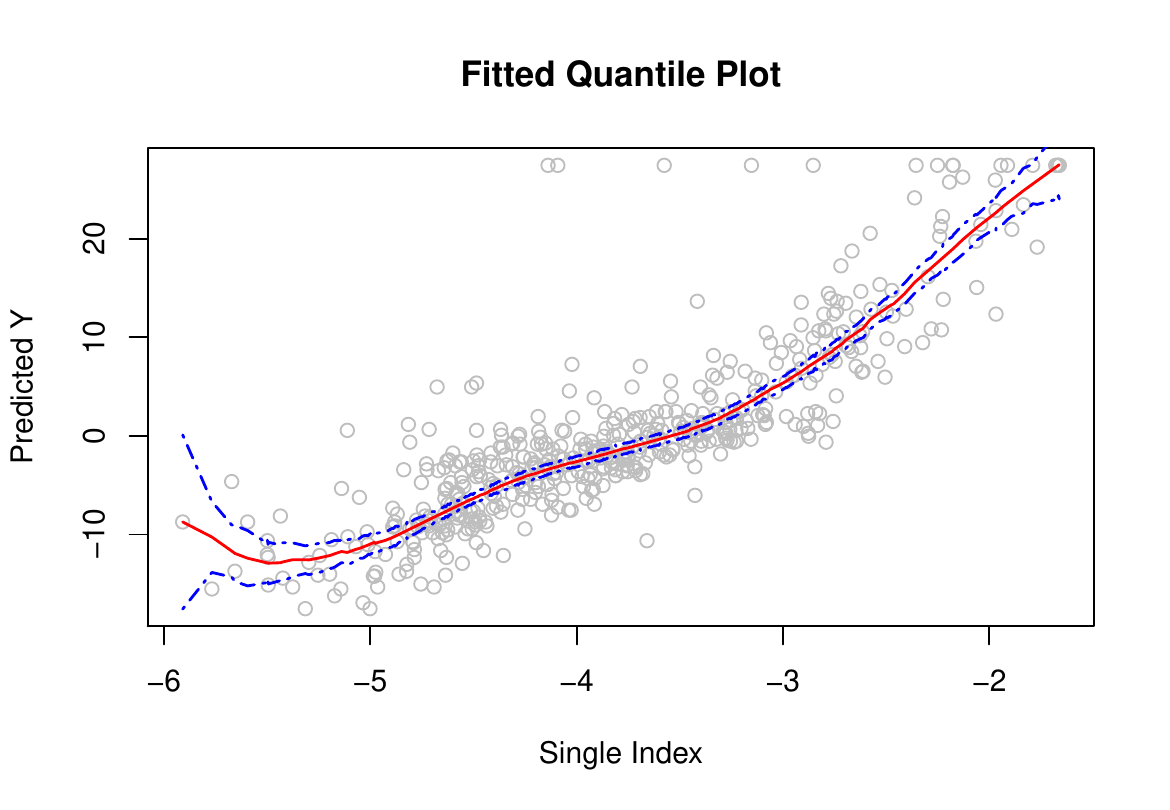
\includegraphics[width=\linewidth]{RJ-2024-038_files/figure-latex/unnamed-chunk-3-1} 

}

\caption{Histogram of values sampled from a gamma distribution, and corresponding standardised values.}\label{fig:unnamed-chunk-3}
\end{figure}

The argument \texttt{index\_type} in \texttt{std\_index()} specifies which type of standardised index should be constructed from the estimated distribution. This must be one of \texttt{"normal"} (the default), \texttt{"prob01"}, or \texttt{"prob11"}, corresponding respectively to the definitions of normal, probability, and bounded standardised indices defined in the previous section.

The \texttt{dist} argument specifies how the distribution \(F\) will be estimated from \texttt{x\_ref}. The default is to use the empirical distribution of \texttt{x\_ref} (Equation 1). To accurately estimate \(F\), the empirical distribution requires a sufficiently large archive, and a warning is therefore returned if the length of \texttt{x\_ref} is smaller than 100. An error message is returned if the distribution support does not align with the data; for example, if a distribution with support \([0, \infty)\) is chosen while the data contains negative values.

Information about the distribution fit, including estimated parameters and goodness-of-fit statistics, can be returned by setting \texttt{return\_fit\ =\ TRUE}; the default is \texttt{return\_fit\ =\ FALSE}. If \texttt{return\_fit\ =\ TRUE}, the output of \texttt{std\_index()} is a list containing the time series of standardised indices (\texttt{si}), the estimated distribution parameters (\texttt{params}), and a named vector containing properties of the model fit (\texttt{fit}); this includes the number of observations used to estimate the distribution, the number and percentage of \texttt{NA} values in the data, the Akaike Information Criterion (AIC) value, and the p-value of the Kolmogorov-Smirnov test that the distribution correctly fits the data; a small p-value provides evidence to suggest that the distribution does not fit the data.

The distribution fitting is performed using \texttt{fit\_dist()}, which is essentially a wrapper for \texttt{fitdist()} in the \CRANpkg{fitdistrplus} package, along with extensions that are relevant for the construction of standardised indices. The \texttt{fit\_dist()} function is also exported by \CRANpkg{SEI}, and further details can be found on the associated help page. Parameters of the distributions (if any) are estimated by default using maximum likelihood estimation, though many other estimation techniques, including method of moments and method of L-moments, can be employed by changing the \texttt{method} argument. Other arguments to \texttt{fitdist()} can be specified as variable arguments \texttt{...}.

\hypertarget{non-stationary-distributions}{%
\subsection{Non-stationary distributions}\label{non-stationary-distributions}}

The default is to estimate a non-stationary distribution from the data in \texttt{x\_ref}. However, non-stationary distributions can be estimated via the GAMLSS framework by inputting a data frame of predictor variables in \texttt{preds\_ref}. This data frame should have the same number of rows as the length of \texttt{x\_ref}, with each column representing a separate predictor variable. Similarly, \texttt{preds\_new} should be a data frame containing the same predictor variables as \texttt{preds\_ref} (with the same column names), but with rows corresponding to the entries of \texttt{x\_new}. The \texttt{std\_index()} function then estimates the non-stationary distribution by calling \texttt{gamlss()} from the \CRANpkg{gamlss} package. The model assumes that the location parameter of the distribution depends linearly on all predictors in \texttt{preds\_ref}. Relationships between the predictors and other distribution parameters, as well as other optional arguments to \texttt{gamlss()}, can again be applied using \texttt{...}.

For example, consider observations drawn from a normal distribution whose mean and standard deviation both increase over time.

\begin{verbatim}
N <- 1000
t <- seq(10, 20, length.out = N)
x <- rnorm(N, mean = t, sd = exp(t/10))
\end{verbatim}

The underlying distribution of these values can be estimated both with and without including a trend in the location and scale parameters of the distribution. Note that \texttt{sigma.formula} is an optional argument to \texttt{gamlss()} that allows the scale parameter of the distribution to depend on predictors.

\begin{verbatim}
preds <- data.frame(t = t)
# standardised indices without trend
si_st <- std_index(x, dist = "norm")
# standardised indices with trend in mean
si_nst <- std_index(x, dist = "norm", preds_new = preds)
# standardised indices with trend in mean and sd
si_nst2 <- std_index(x, dist = "norm", preds_new = preds, sigma.formula = ~ t)
\end{verbatim}

Figure 2 displays the time series of standardised indices corresponding to these values under three different assumptions: there is no trend, there is a linear trend in the mean but not the standard deviation of the distribution, and there is a trend in both the mean and standard deviation. When the trend is not included, higher index values unsurprisingly occur at higher time points, and the variation of the indices also increases in time. If a trend is included in the mean of the distribution, then the standardised indices do not increase in time, but still become more variable. If a trend is included in both the mean and the standard deviation, then the index values become stationary.

\begin{figure}

{\centering 
\includegraphics[width=\linewidth]{RJ-2024-038_files/figure-latex/unnamed-chunk-4-1} 

}

\caption{Standardised indices corresponding to a time series of values drawn from a non-stationary normal distribution. Results are shown when the estimated normal distribution does and does not include a trend.}\label{fig:unnamed-chunk-4}
\end{figure}

\hypertarget{grouping}{%
\subsection{Grouping}\label{grouping}}

Rather than estimating one distribution across all observations, whether dependent on predictors or not, the variable of interest may have a distribution that changes in different subsets of the data. These subsets could correspond to different seasons, for example. Standardised indices corresponding to different distributions can be derived from \texttt{std\_index()} via the \texttt{gr\_new} and \texttt{gr\_ref} arguments. These should be factor vectors of the same length as \texttt{x\_new} and \texttt{x\_ref} respectively, with each factor corresponding to a different subset of the data from which a distribution should be estimated. The values in \texttt{x\_ref} are stratified according to \texttt{gr\_ref}, and a separate distribution is estimated from each subset; the values in \texttt{x\_new} are then stratified according to \texttt{gr\_new}, and the distribution corresponding to each factor level is applied to the subset of values in \texttt{x\_new} that correspond to the same level. The factor levels in \texttt{x\_new} and \texttt{x\_ref} should therefore be the same. In particular, \texttt{x\_new} should not contain any levels that are not also present in \texttt{x\_ref}, since in this case there would be no data in \texttt{x\_ref} from which to estimate the relevant distribution. This returns an error.

Non- and semi-parametric distributions can flexibly adapt to situations where the shape of the distribution changes within the different subsets of the data. However, if a large number of factor levels are present in \texttt{x\_ref} and \texttt{x\_new}, then the amount of data to estimate the distributions can become small. To counteract this, the \texttt{dist} argument in \texttt{std\_index()} can be a vector of the same length as the number of levels in \texttt{gr\_ref}. The first element of \texttt{dist} denotes the distribution to be fit to the data corresponding to the first factor of \texttt{gr\_ref}, and so on. Currently, for non-stationary distributions, the predictors do not depend on the grouping, and thus the same relationship between the variable of interest and the predictors must be assumed for each subset.

\hypertarget{censoring}{%
\subsection{Censoring}\label{censoring}}

The theory underlying standardised indices in Section 2 relies on the variable of interest being continuous, and the distributions available in \CRANpkg{SEI} are therefore also all continuous. However, standardised indices may also be informative when the variable of interest is not continuous. A particular example is when the variable is censored; that is, it is bounded either above or below (or both), with positive probability of being exactly equal to the boundary points. Precipitation, for example, is censored below at zero.

Depending on how they are used, the definition of standardised indices may need to be adjusted to account for the censoring. This has been considered, for example, by \cite{StaggeEtAl2015}. How to deal with censored variables is discussed in detail in the appendix. Censored data can be handled in \CRANpkg{SEI} using the \texttt{lower}, \texttt{upper}, and \texttt{cens} arguments in \texttt{std\_index()}: \texttt{lower} and \texttt{upper} specify the lower and upper bounds of the data, respectively, while \texttt{cens} determines the method used to address the censoring. The available methods are outlined in the appendix.

\hypertarget{time-series-manipulations}{%
\subsection{Time series manipulations}\label{time-series-manipulations}}

The remaining arguments of \texttt{std\_index()} are only applicable when \texttt{x\_new} and \texttt{x\_ref} are time series, rather than vectors, since they all involve manipulations based on the date of the data. For example, the argument \texttt{moving\_window} can be used to calculate standardised indices using a moving window. In this case, \texttt{x\_ref} is updated for each observation in \texttt{x\_new} so that it contains the previous \texttt{moving\_window} (an integer) observations in the time series; the indices are therefore determined relative to recently observed values. The argument \texttt{window\_scale} specifies the timescale that \texttt{moving\_window} refers to. For example, setting \texttt{moving\_window\ =\ 10} and \texttt{window\_scale\ =\ "days"} would calculate standardised indices using a moving window of length 10 days.

If \texttt{moving\_window} is specified but \texttt{window\_scale\ =\ NULL}, then it is assumed that the units of \texttt{moving\_window} correspond to the timescale of \texttt{x\_new}. If the time difference between consecutive observations is consistent throughout the time series, then this can be determined automatically within \texttt{std\_index()}. Alternatively, and more robustly, it can be specified by the user using the \texttt{timescale} argument. This (and \texttt{window\_scale}) must be one of \texttt{"mins"}, \texttt{"hours"}, \texttt{"days"}, \texttt{"weeks"}, \texttt{"months"}, or \texttt{"years"}.

If the original time series contains, say, hourly data, but the time series of standardised indices is desired on a different timescale, then the \texttt{rescale} argument can be used to rescale the data. This must also be one of the timescales listed above. By default, \texttt{std\_index()} assumes the sum of the values should be returned when rescaling. For example, if interest is on precipitation accumulations, then converting hourly data to daily data will return the daily aggregations. However, alternative rescaling could also be performed using the \texttt{rescale\_fun} argument, which is a function specifying what operation to perform over the aggregated data. If \texttt{rescale\_fun\ =\ "mean"} or \texttt{rescale\_fun\ =\ "max"}, for example, then the daily (or weekly, monthly, etc) mean or maximum would be provided, respectively, in place of the hourly data.

Similarly, the \texttt{agg\_period} argument can be used to aggregate data across multiple time steps. Like \texttt{moving\_window} and \texttt{window\_scale}, \texttt{agg\_period} is an integer representing the number of previous time steps over which the data should be aggregated, while \texttt{agg\_scale} specifies the timescale of the aggregation period, which is by default assumed to be the timescale of the data. The argument \texttt{agg\_fun} represents the function used to aggregate the data over the aggregation period.

This differs from \texttt{rescale} in the following way. If we want to convert a time series of daily observations to a time series of weekly indices, then we can use \texttt{rescale\ =\ "weeks"} (and \texttt{timescale\ =\ "days"}). On the other hand, if we set \texttt{agg\_period\ =\ 1} and \texttt{agg\_scale\ =\ "weeks"}, then we get a daily time series of weekly aggregated data.

To perform the rescaling, \texttt{std\_index()} calls one of the \CRANpkg{xts} functions \texttt{apply.daily}, \texttt{apply.weekly}, \texttt{apply.monthly}, \texttt{apply.quarterly}, and \texttt{apply.yearly}, alongside the argument \texttt{rescale\_fun}. To perform the aggregation, \texttt{std\_index()} uses the function \texttt{aggregate\_xts()}, which is additionally exported by \CRANpkg{SEI}.

\begin{verbatim}
aggregate_xts(
  x,
  agg_period = 1,
  agg_scale = c("days", "mins", "hours", "weeks", "months", "years"),
  agg_fun = "sum",
  timescale = c("days", "mins", "hours", "weeks", "months", "years"),
  na_thres = 10
)
\end{verbatim}

The interpretation of the arguments is equivalent to in the discussion above: \texttt{x} represents the \CRANpkg{xts} time series to be aggregated, \texttt{agg\_period} and \texttt{agg\_scale} are the length and time scale of the aggregation period, \texttt{agg\_fun} is the function used in the aggregation, and \texttt{timescale} is the time scale of \texttt{x}. The final argument \texttt{na\_thres} represents the maximum proportion of values that can be missing (i.e.~\texttt{NA}) in the aggregation period, before the aggregation itself returns \texttt{NA}. For example, if 23 hours of precipitation accumulations are missing on one day so that only one hourly accumulation is available, this sole observation is not representative of the daily accumulation. By default, \texttt{NA} is returned if more than 10\% of the values in the aggregation period are missing.

\hypertarget{plotting-standardised-indices}{%
\subsection{Plotting standardised indices}\label{plotting-standardised-indices}}

To visualise the indices, \CRANpkg{SEI} includes the \texttt{plot\_sei()} function.

\begin{verbatim}
plot_sei(
  x,
  type = c("ts", "hist", "bar"),
  title = NULL,
  lab = "Std. Index",
  xlims = NULL,
  ylims = NULL,
  n_bins = 30
)
\end{verbatim}

The argument \texttt{x} is either a vector or an \CRANpkg{xts} time series object that contains the index values to be displayed. This function can either be used to plot a time series of the values (\texttt{type\ =\ "ts"}), a histogram (\texttt{type\ =\ "hist"}), or a bar plot (\texttt{type\ =\ "bar"}). If \texttt{type\ =\ "hist"}, the function is essentially a wrapper for \texttt{geom\_histogram()} in \CRANpkg{ggplot2}. The histogram and bar plot both display the distribution of the values in \texttt{x}. The histogram is particularly useful when superimposing a density onto the histogram, while the bar plot is also made available since it can be more robust when the data in \texttt{x} is bounded. Here, \texttt{n\_bins} can be used to specify the number of bins in the plot.

Additional aspects of the plot can be specified using \texttt{title}, \texttt{lab}, \texttt{xlims} and \texttt{ylims}. For the time series plot, \texttt{lab} refers to the label of the y-axis, whereas it corresponds to the x-axis label of the histogram and bar plot.

\hypertarget{drought-definitions}{%
\subsection{Drought definitions}\label{drought-definitions}}

Having obtained a time series of standardised indices, one might wish to perform an analysis of shortages, or droughts, in the variable of interest. As discussed, this can be achieved using standardised indices with the definitions of droughts in Table 1. To facilitate such analyses, the \texttt{get\_drought()} function takes a time series or vector \texttt{x} as input, and outputs a dataframe containing information regarding drought occurrences and characteristsics.

\begin{verbatim}
get_drought(
  x,
  thresholds = c(1.28, 1.64, 1.96),
  exceed = TRUE,
  cluster = 0,
  lag = NULL
)
\end{verbatim}

The argument \texttt{thresholds} is a vector containing the thresholds used to define the droughts; by default, these correspond to the 90\(^{th}\), 95\(^{th}\), and 97.5\(^{th}\) percentiles of a standard normal distribution. It is also assumed by default that a drought is defined when the standardised indices exceed these thresholds. This can be specified using the \texttt{exceed} argument. If a drought should instead correspond to an instance where the indices fall below the given thresholds, \texttt{exceed} should be \texttt{FALSE}.

When defining meteorological droughts, it is often common to introduce a lag such that the drought does not end when the standardised index no longer exceeds the drought threshold, but rather when the index falls below a lower threshold (such as zero for the SPI) \citep[e.g.][]{MckeeEtAl1993}. This accounts for cases where there are small fluctuations in the index around the drought threshold, classing this as one persistent drought rather than several shorter droughts. This can be implemented in \CRANpkg{SEI} by specifying the \texttt{lag} argument, which is a numeric value denoting the weaker threshold to use when lagging the indices.

Alternatively, these fluctuations could be avoided by clustering together drought events separated by a small number of days \citep[e.g.][]{OteroEtAl2022}. The number of days between which drought events should be clustered can be specified via the \texttt{cluster} argument in \texttt{get\_drought()}. The default is to not cluster droughts.

As an example, consider the previous time series of standardised indices corresponding to a random sample from a gamma distribution.

\begin{verbatim}
head(get_drought(x_std))
\end{verbatim}

\begin{verbatim}
#>             x ins occ dur mag
#> 1 -1.12290688   0   0   0   0
#> 2 -0.43622340   0   0   0   0
#> 3 -0.87195389   0   0   0   0
#> 4  0.08515807   0   0   0   0
#> 5  0.81832146   0   0   0   0
#> 6  0.78384046   0   0   0   0
\end{verbatim}

The output is a dataframe containing the original vector or time series, as well as four additional columns: the intensity (\texttt{ins}), which corresponds to the category of drought, a higher value referring to a more severe drought category; the occurrence (\texttt{occ}), which corresponds to the intensity being higher than zero; the duration (\texttt{dur}), which provides the number of consecutive time steps that are in a drought state; and the drought magnitude (\texttt{mag}), which is the sum of all indices within the drought event \citep[see][for details]{MckeeEtAl1993}. If only one threshold is used to define a drought, rather than the three used in Table 1, then the intensity is equivalent to the occurrence, and is therefore not returned.

\hypertarget{applications}{%
\section{Applications}\label{applications}}

\hypertarget{renewable-energy-production}{%
\subsection{Renewable energy production}\label{renewable-energy-production}}

Consider an application of standardised indices to renewable energy production in Europe. Hourly time series of wind and solar power generation are publicly available for 27 European countries at \url{https://researchdata.reading.ac.uk/275/} \citep[see][for details]{BloomfieldEtAl2020}. A subset of this data corresponding to production in 2019 can be accessed from \CRANpkg{SEI} using

\begin{verbatim}
data("data_supply", package = "SEI")
head(data_supply)
\end{verbatim}

\begin{verbatim}
#>                  date country        PWS
#> 1 2019-01-01 00:00:00 Austria 0.07823861
#> 2 2019-01-01 01:00:00 Austria 0.05330285
#> 3 2019-01-01 02:00:00 Austria 0.06773745
#> 4 2019-01-01 03:00:00 Austria 0.09971320
#> 5 2019-01-01 04:00:00 Austria 0.18676895
#> 6 2019-01-01 05:00:00 Austria 0.29001299
\end{verbatim}

The dataframe \texttt{data\_supply} contains a \texttt{POSIXct} time series of dates, along with the corresponding country and wind and solar power production (\texttt{PWS}). The units of the production are Gigawatt hours (GWh).

For concision, we restrict attention here to renewable energy production in Germany.

\begin{verbatim}
de_supply_h <- subset(data_supply, country == "Germany")
de_supply_h <- xts::xts(de_supply_h$PWS, de_supply_h$date) # convert to xts
\end{verbatim}

This can be rescaled from hourly to daily or weekly time series using \CRANpkg{xts} functionality.

\begin{verbatim}
de_supply_d <- xts::apply.daily(de_supply_h, "sum")    # daily data
de_supply_w <- xts::apply.weekly(de_supply_h, "sum")   # weekly data
\end{verbatim}

These time series of renewable energy production in Germany can be visualised using the \texttt{plot\_sei()} function. Figure 3 demonstrates that all three time series display the same patterns, though the weekly time series removes the hourly and daily fluctuations.

\begin{verbatim}
lab <- "Renewable Energy Production (GWh)"
plot_h <- plot_sei(de_supply_h, lab = lab, title = "Hourly")
plot_d <- plot_sei(de_supply_d, lab = lab, title = "Daily")
plot_w <- plot_sei(de_supply_w, lab = lab, title = "Weekly")
grid.arrange(plot_h, plot_d, plot_w, nrow = 1)
\end{verbatim}

\begin{figure}

{\centering 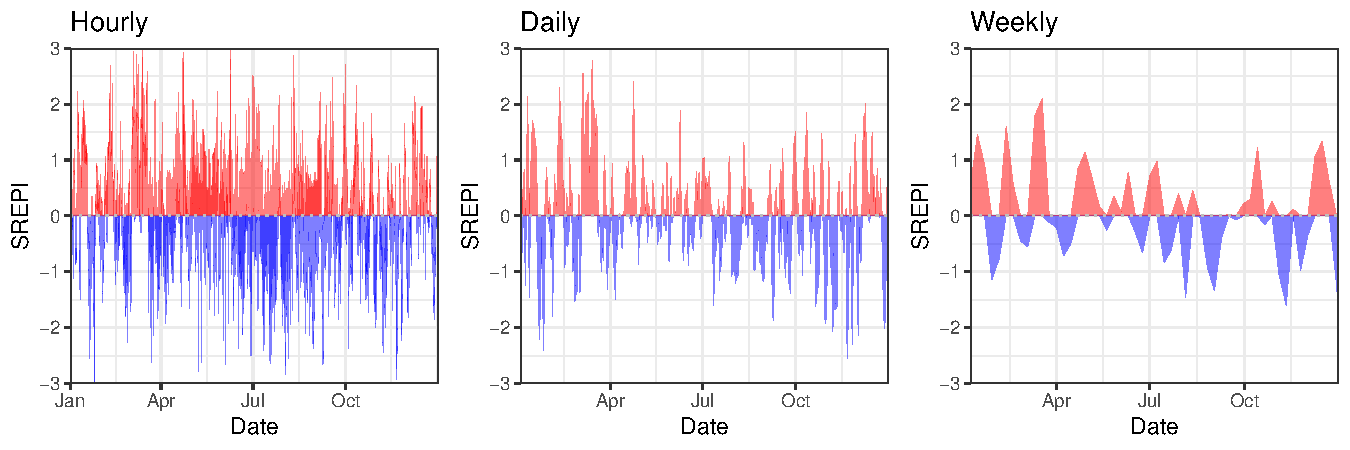
\includegraphics[width=\linewidth]{RJ-2024-038_files/figure-latex/unnamed-chunk-5-1} 

}

\caption{Time series of 2019 renewable energy production in Germany at hourly, daily, and weekly time scales.}\label{fig:unnamed-chunk-5}
\end{figure}

The raw renewable energy production values can be transformed to a standardised index using \texttt{std\_index()}.

\begin{verbatim}
srepi_h <- std_index(de_supply_h)
srepi_d <- std_index(de_supply_d)
srepi_w <- std_index(de_supply_w, dist = "kde")
\end{verbatim}

Following, \cite{AllenOtero2023}, we refer to this as the standardised renewable energy production index (SREPI). Time series of hourly, daily, and weekly SREPI values are presented in Figure 4.

\begin{verbatim}
lab <- "SREPI"
ylims <- c(-3, 3)
plot_h <- plot_sei(srepi_h, lab = lab, ylims = ylims, title = "Hourly")
plot_d <- plot_sei(srepi_d, lab = lab, ylims = ylims, title = "Daily")
plot_w <- plot_sei(srepi_w, lab = lab, ylims = ylims, title = "Weekly")
grid.arrange(plot_h, plot_d, plot_w, nrow = 1)
\end{verbatim}

\begin{figure}

{\centering 
\includegraphics[width=\linewidth]{RJ-2024-038_files/figure-latex/unnamed-chunk-6-1} 

}

\caption{Time series of 2019 SREPI values in Germany at hourly, daily, and weekly time scales.}\label{fig:unnamed-chunk-6}
\end{figure}

In this case, the reference data \texttt{x\_ref} is assumed to be the input time series itself, meaning the indices are calculated relative to this input data. By default, \texttt{std\_index()} returns normal indices (rather than probability or bounded indices), and estimates the distribution of the renewable energy production using the empirical distribution. This returns a warning for the weekly data, since there are fewer than 100 weekly production values in the time series. Instead, for weekly data, we estimate the distribution of production values using kernel density estimation (\texttt{dist\ =\ "kde"}). Alternative distributions could be implemented by changing the \texttt{dist} argument in \texttt{std\_index()}.

While these indices are created by standardising the respective hourly, daily, and weekly time series of raw production values, they could all be obtained from the original hourly time series by specifying the \texttt{rescale} argument in \texttt{std\_index()}.

\begin{verbatim}
z <- std_index(de_supply_h, rescale = "days")
all.equal(srepi_d, z)
\end{verbatim}

\begin{verbatim}
#> [1] TRUE
\end{verbatim}

By default, the \texttt{plot\_sei()} function displays the time series of input values. However, by specifying \texttt{type\ =\ "hist"} (rather than the default \texttt{type\ =\ "ts"}), this function can additionally be used to plot a histogram of the input values. An example of this for the daily data production and corresponding SREPI values is presented in Figure 5. As discussed in Section 3, such a plot can be used to validate the distributional assumptions made when calculating the indices. While the raw renewable energy production follows a heavily skewed distribution, the SREPI values resemble a sample from a standard normal distribution, suggesting the empirical distribution function is appropriate in this example. If probability or bounded indices were used, then the histogram of SREPI values should be flat, rather than normal. This is illustrated in Figure 6.

\begin{figure}

{\centering 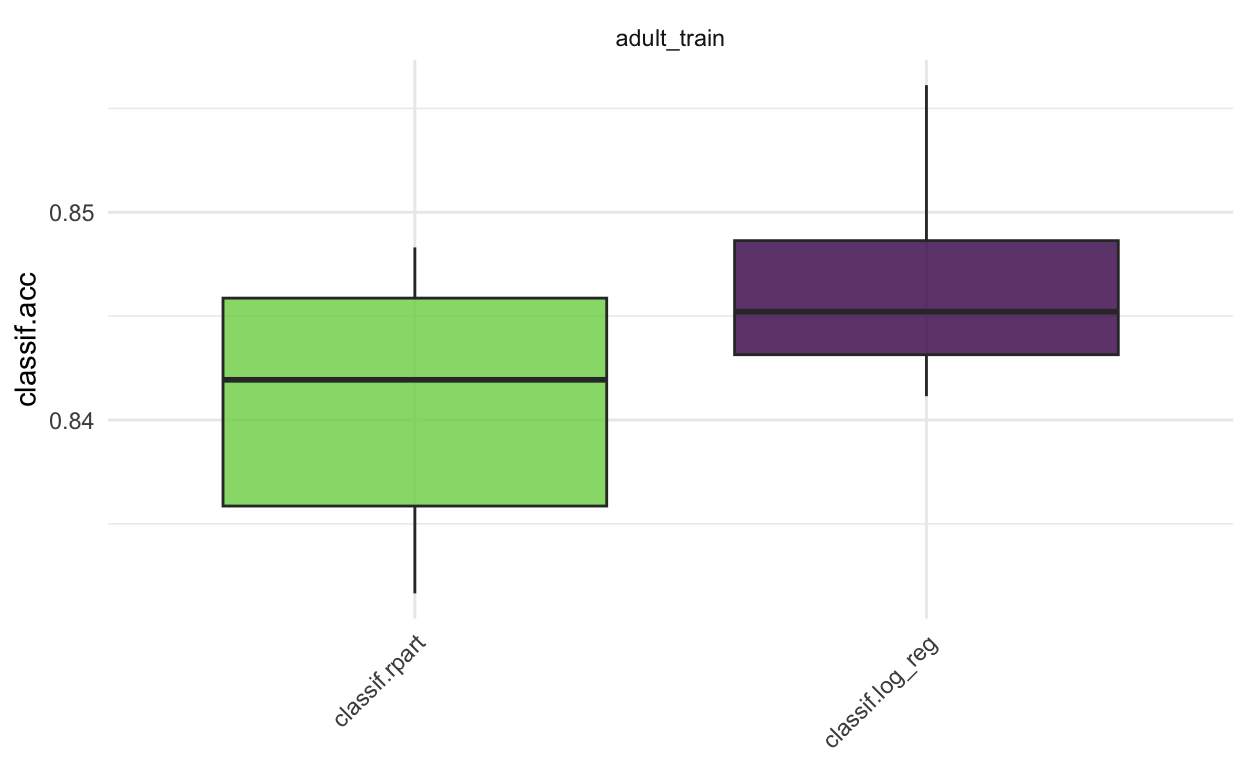
\includegraphics[width=\linewidth]{RJ-2024-038_files/figure-latex/unnamed-chunk-7-1} 

}

\caption{Histogram of 2019 daily renewable energy production and SREPI values in Germany.}\label{fig:unnamed-chunk-7}
\end{figure}

\begin{figure}

{\centering 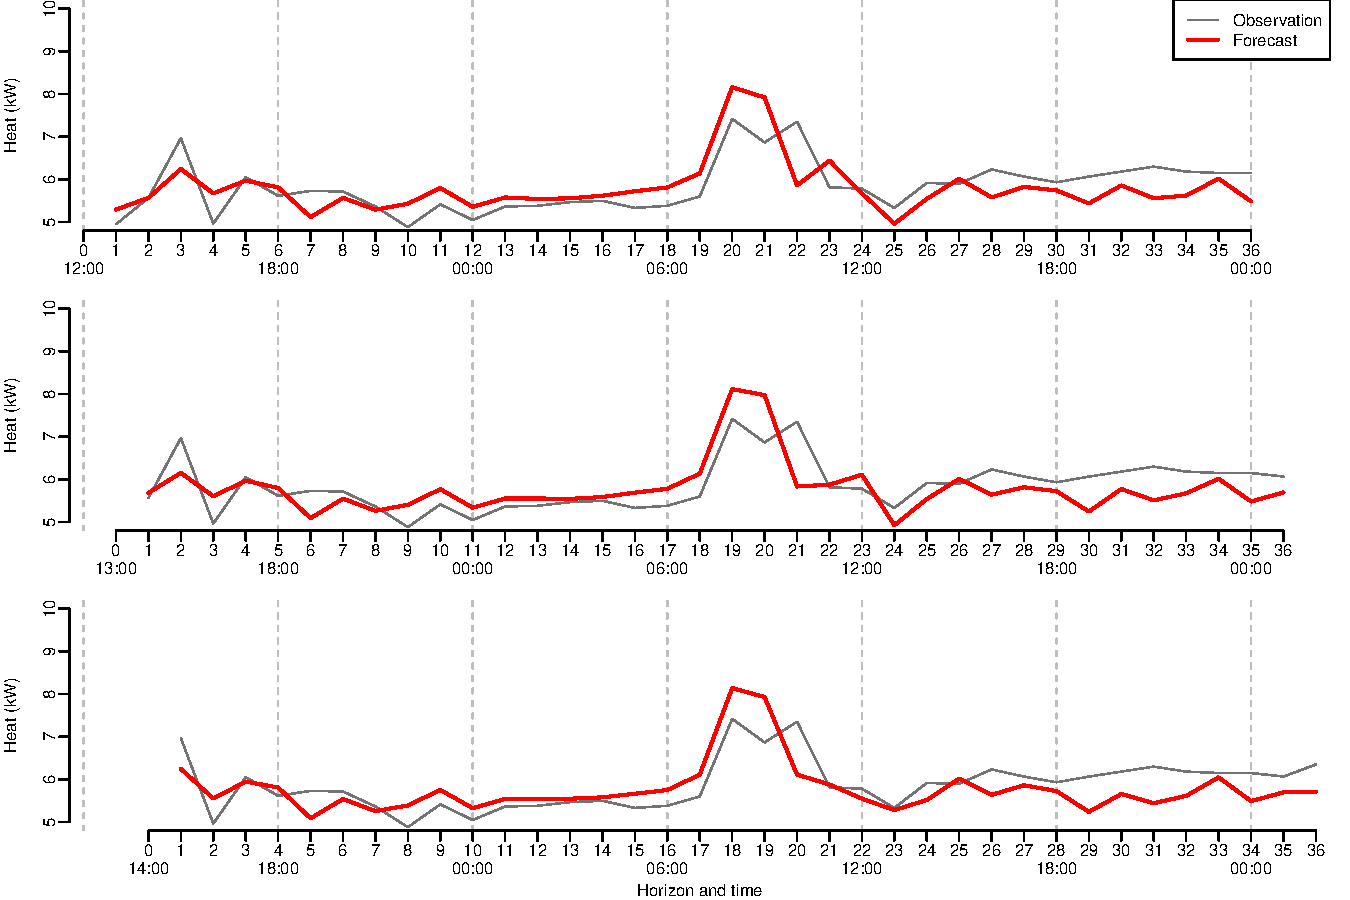
\includegraphics[width=\linewidth]{RJ-2024-038_files/figure-latex/unnamed-chunk-8-1} 

}

\caption{Histogram of 2019 daily renewable energy production and SREPI values in Germany, where the indices are probability and bounded indices.}\label{fig:unnamed-chunk-8}
\end{figure}

Finally, the \CRANpkg{SEI} package additionally allows shortages or drought characteristics of the time series to be assessed. In this case, an energy supply drought could occur if the renewable energy production is low compared to previously observed values \citep{AllenOtero2023}. This corresponds to a low SREPI. As in Table 1, we define three categories of droughts, each defined using increasing thresholds of the SREPI. The function \texttt{get\_drought()} can then be used to obtain a time series of drought occurrences, intensities, durations, and magnitudes.

\begin{verbatim}
thresholds <- qnorm(c(0.1, 0.05, 0.025)) # -1.28, -1.64, -1.96
drought_df <- get_drought(srepi_d, thresholds, exceed = F)
\end{verbatim}

From the dataframe \texttt{drought\_df}, it is straightforward to analyse the properties of these drought events. For example, we can list the frequency that a moderate, severe, or extreme drought event occurs

\begin{verbatim}
num_ev <- table(drought_df$ins)
names(num_ev) <- c("None", "Moderate", "Severe", "Extreme")
print(num_ev)
\end{verbatim}

\begin{verbatim}
#>     None Moderate   Severe  Extreme 
#>      330       18        9        8
\end{verbatim}

we could display the relative frequency of drought durations

\begin{verbatim}
table(drought_df$dur[drought_df$dur > 0])
\end{verbatim}

\begin{verbatim}
#> 
#>  1  2  3 
#> 11  3  6
\end{verbatim}

or we could calculate the average drought magnitude

\begin{verbatim}
mean(drought_df$mag[drought_df$mag != 0])
\end{verbatim}

\begin{verbatim}
#> [1] 2.985504
\end{verbatim}

These are just simple examples of analyses that could be performed using the output of \texttt{get\_drought()}. For a more thorough analysis, readers are referred to \cite{AllenOtero2023}.

\hypertarget{wind-speed}{%
\subsection{Wind speed}\label{wind-speed}}

Consider now a second application of standardised indices to weather and climate variables. While standardised indices are most commonly used to construct the SPI and SPEI, they can also be applied to other climate variables (see Section 1 for examples). In this section, we use the framework discussed herein to define standardised wind speed indices. Monitoring wind speed is crucial in many applications, including aviation safety, renewable energy planning, and the design and insurance of infrastructure.

Hourly estimates of near-surface (10m) wind speed are publicly available for several European countries between 1979 and 2019 \citep{HersbachEtAl2023}. As in \cite{OteroEtAl2022b}, we aggregate these wind speeds to get daily nationwide averages. Consistent with the previous application to renewable energy production, the analysis is restricted to Germany, and this subset of data is available from \CRANpkg{SEI}. For clarity of visualisation, the following analysis is limited to the three year period between 2017 and 2019.

\begin{verbatim}
data("data_wind_de", package = "SEI")
data_wind_de <- subset(data_wind_de, format(date, "%Y") >= 2017)
head(data_wind_de)
\end{verbatim}

\begin{verbatim}
#>             date   wsmean
#> 13881 2017-01-01 3.461528
#> 13882 2017-01-02 3.479744
#> 13883 2017-01-03 5.391327
#> 13884 2017-01-04 6.801471
#> 13885 2017-01-05 3.822558
#> 13886 2017-01-06 2.101849
\end{verbatim}

As before, the data can be rescaled using \CRANpkg{xts} functionality to obtain time series of the weekly and monthly average wind speed in Germany. We label the resulting daily, weekly, and monthly time series \texttt{de\_wind\_d}, \texttt{de\_wind\_w}, and \texttt{de\_wind\_m}, respectively, all of which are \CRANpkg{xts} objects. These time series are displayed using \texttt{plot\_sei()} in Figure 7.

\begin{verbatim}
lab <- "Wind speed (m/s)"
ylims <- c(0, 8)
plot_ws_d <- plot_sei(de_wind_d, lab = lab, ylims = ylims, title = "Daily")
plot_ws_w <- plot_sei(de_wind_w, lab = lab, ylims = ylims, title = "Weekly")
plot_ws_m <- plot_sei(de_wind_m, lab = lab, ylims = ylims, title = "Monthly")
grid.arrange(plot_ws_d, plot_ws_w, plot_ws_m, nrow = 1)
\end{verbatim}

\begin{figure}

{\centering 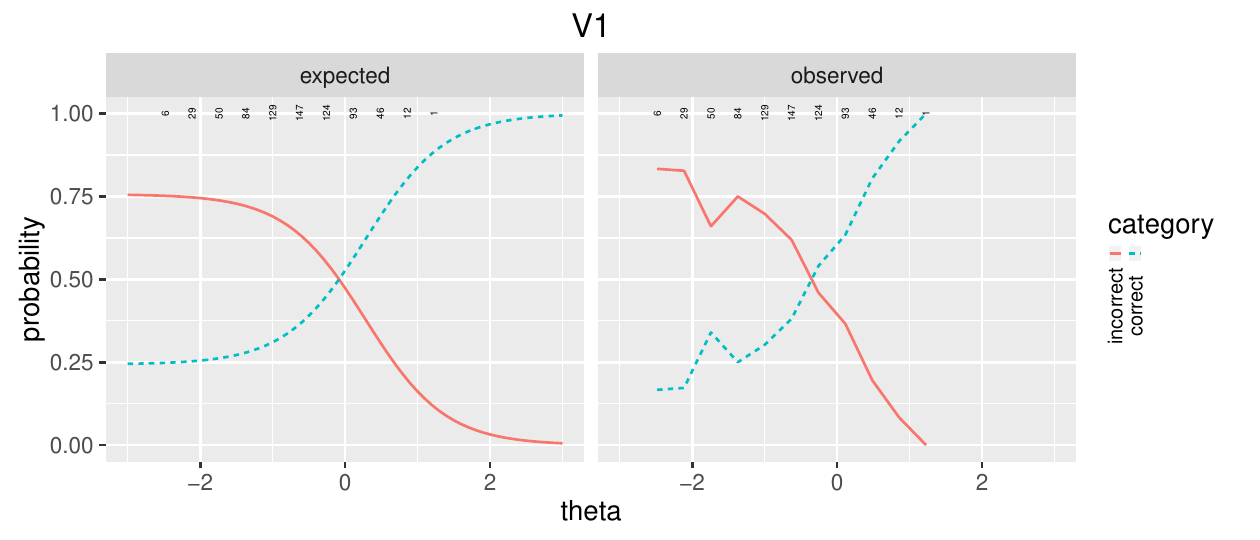
\includegraphics[width=\linewidth]{RJ-2024-038_files/figure-latex/unnamed-chunk-9-1} 

}

\caption{Daily, weekly and monthly time series of average wind speed in Germany between 2017 and 2019.}\label{fig:unnamed-chunk-9}
\end{figure}

The raw data can be transformed to a time series of standardised indices using \texttt{std\_index()}. As discussed, constructing standardised indices requires estimating the distribution of the variable of interest. While we argue that the empirical distribution provides a flexible means to achieve this, we demonstrate in this application how the \CRANpkg{SEI} package allows parametric distributions to be used for this purpose.

Various distributions can be fit to the daily wind speeds using the \texttt{fit\_dist()} function. Consider, for example, a gamma distribution, log-normal distribution, and Weibull distribution.

\begin{verbatim}
out_gamma <- fit_dist(data_wind_de$wsmean, dist = "gamma")
out_lnorm <- fit_dist(data_wind_de$wsmean, dist = "lnorm")
out_weibull <- fit_dist(data_wind_de$wsmean, dist = "weibull")
\end{verbatim}

The three distributions can be compared with respect to their AIC, which is output from \texttt{fit\_dist()}.

\begin{verbatim}
aic_vec <- c(out_gamma$fit['aic'],
             out_lnorm$fit['aic'],
             out_weibull$fit['aic'])
names(aic_vec) <- c("Gamma", "Log-normal", "Weibull")
print(aic_vec)
\end{verbatim}

\begin{verbatim}
#>      Gamma Log-normal    Weibull 
#>   3278.268   3231.083   3443.914
\end{verbatim}

The AIC provides a measure of distributional fit whilst also accounting for model complexity, with a smaller value indicating a better bit. The AIC values above suggest that the log-normal distribution provides the best fit to the data, while the Weibull distribution provides the worst fit.

This can be verified by looking at p-values corresponding to the Kolmogorov-Smirnov test.

\begin{verbatim}
ksp_vec <- c(out_gamma$fit['ks_pval'],
             out_lnorm$fit['ks_pval'],
             out_weibull$fit['ks_pval'])
names(ksp_vec) <- c("Gamma", "Log-normal", "Weibull")
print(round(ksp_vec, 4))
\end{verbatim}

\begin{verbatim}
#>      Gamma Log-normal    Weibull 
#>     0.0047     0.1127     0.0000
\end{verbatim}

The null hypothesis is that the sample of data has been drawn from the parametric distribution. The Kolmogorov-Smirnov test is rejected at the 0.5\% level for both the gamma and Weibull distributions, providing evidence to suggest that these distributions do not accurately describe the data. On the other hand, there is insufficient evidence to reject the null hypothesis that the wind speed data was drawn from a log-normal distribution.

The fit of the three distributions to the data is presented in Figure 8. The \texttt{plot\_sei()} function can be used to plot histograms of the daily wind speeds. Since \texttt{plot\_sei()} returns a \CRANpkg{ggplot2} object, the estimated density functions can be added to the histograms. For example, for the gamma distribution

\begin{verbatim}
x <- seq(0, 9, length.out = length(de_wind_d))
xlab <- "Wind speed (m/s)"
pars_gam <- out_gamma$params

plt_gam <- plot_sei(de_wind_d, type = "hist", lab = xlab, title = "Gamma") +
  geom_line(aes(x = x, y = dgamma(x, pars_gam[1], pars_gam[2])), col = "blue")
\end{verbatim}

\begin{figure}

{\centering 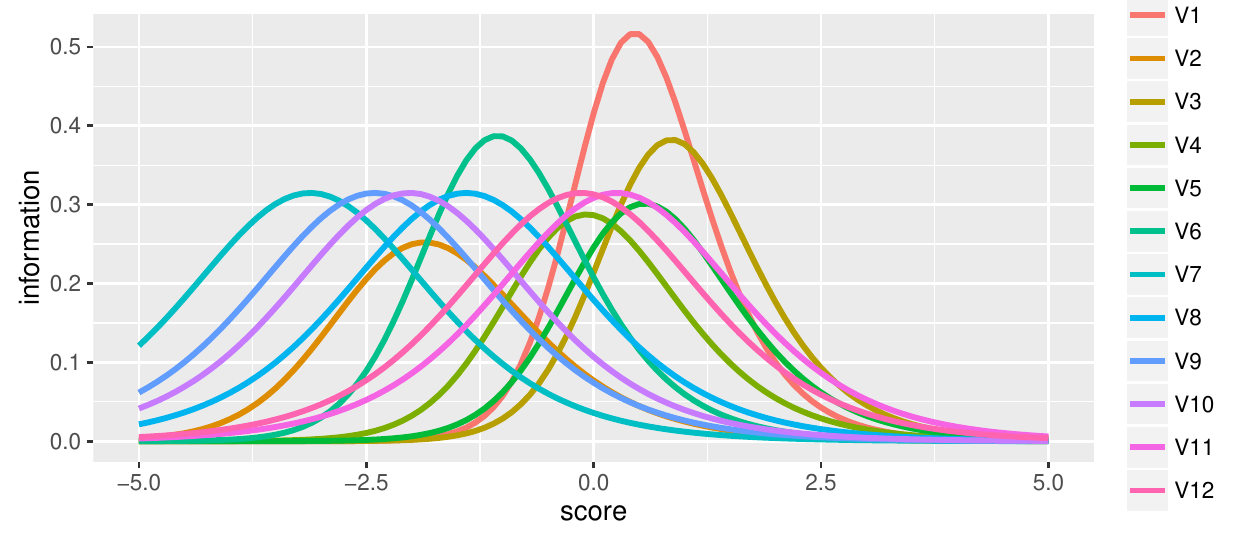
\includegraphics[width=\linewidth]{RJ-2024-038_files/figure-latex/unnamed-chunk-10-1} 

}

\caption{Distribution of daily wind speeds in Germany between 2017 and 2019, along with estimated gamma, log-normal, and Weibull densities.}\label{fig:unnamed-chunk-10}
\end{figure}

Finally, the adequacy of the distributions can also be visualised by plotting a histogram of the standardised indices obtained using the three distributions. The standardised indices can be calculated using the \texttt{std\_index()} function, with the \texttt{dist} argument corresponding to the distribution of interest. When probability indices are used (\texttt{index\_type\ =\ "prob01"}), plotting a histogram of the indices is equivalent to displaying the probability integral transform (PIT) histogram commonly used to assess the fit of probabilistic models.

\begin{verbatim}
sei_ws_gam <- std_index(de_wind_d, dist = "gamma")
sei_ws_lnorm <- std_index(de_wind_d, dist = "lnorm")
sei_ws_weib <- std_index(de_wind_d, dist = "weibull")
\end{verbatim}

Histograms of the standardised indices, constructed using \texttt{plot\_sei()}, are displayed in Figure 9. Similarly to before, a standard normal distribution is superimposed onto the histograms.

\begin{figure}

{\centering 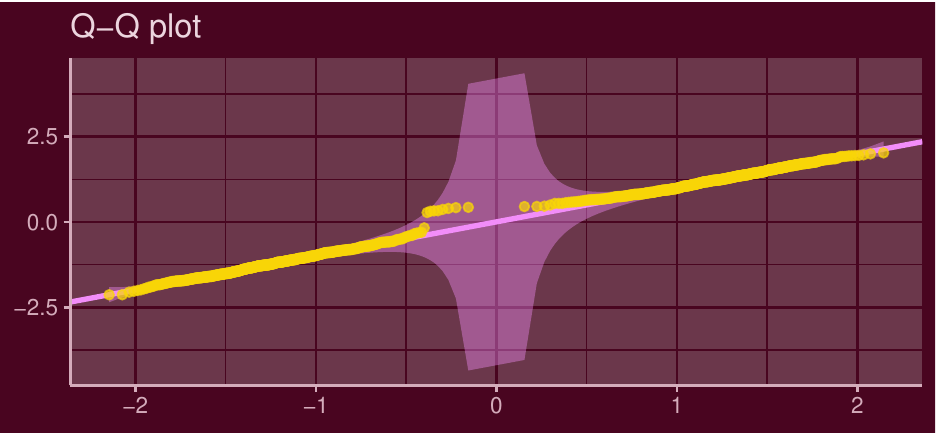
\includegraphics[width=\linewidth]{RJ-2024-038_files/figure-latex/unnamed-chunk-11-1} 

}

\caption{Distribution of standardised wind speed indices (SWSI) constructed using the gamma, log-normal, and Weibull distributions. The standard normal density is displayed in blue.}\label{fig:unnamed-chunk-11}
\end{figure}

As expected, no parametric distribution fits the data perfectly. The standardised wind speed indices constructed using a log-normal distribution appear closer to a standard normal distribution, and this is reinforced by quantile-quantile plots in Figure 10, which compare the quantiles of the SWSI values to the quantiles of a standard normal distribution. This supports the conclusion that the log-normal distribution provides a more accurate fit to the daily wind speed data, which also agrees with previous studies that use this distribution when modelling wind speed \citep[e.g.][]{KolluEtAl2012,BaranLerch2015}.

\begin{figure}

{\centering 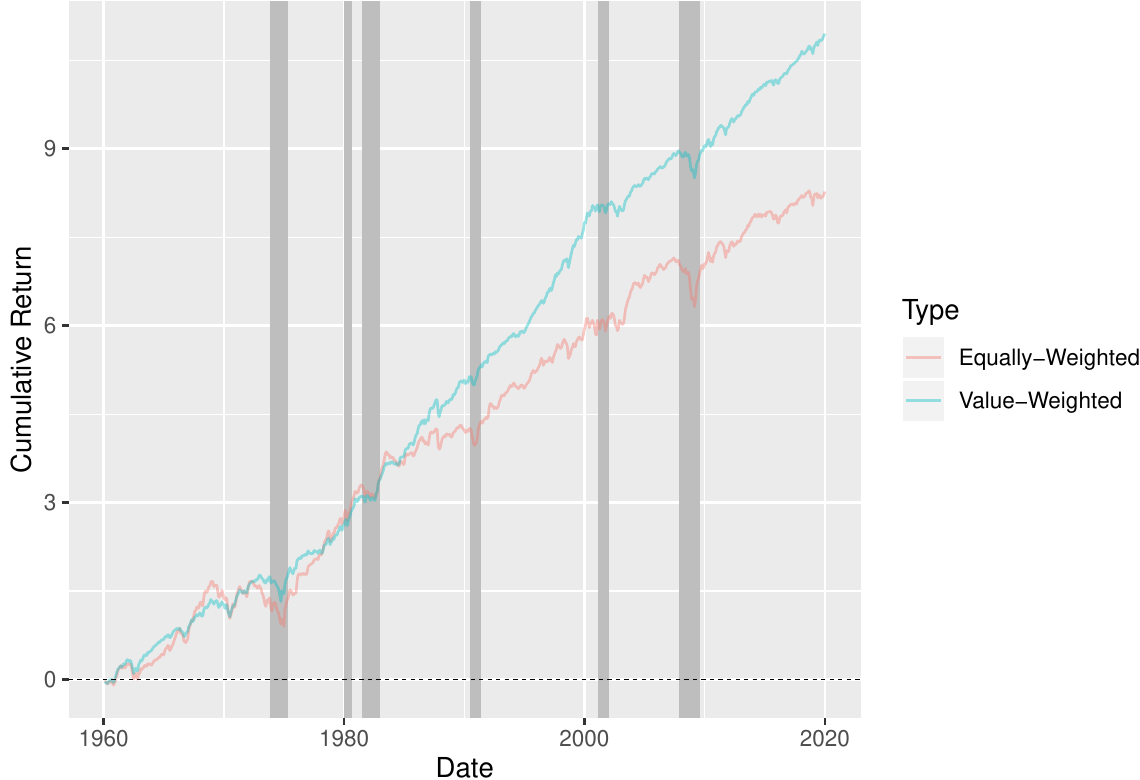
\includegraphics[width=\linewidth]{RJ-2024-038_files/figure-latex/unnamed-chunk-12-1} 

}

\caption{Normal quantile-quantile (qq) plots showing the fit of the standard normal distribution to the distribution of SWSI values.}\label{fig:unnamed-chunk-12}
\end{figure}

Having constructed these wind speed indices, it would be straightforward to conduct an analysis of wind droughts (or extreme wind speeds) using the \texttt{get\_drought()} function in \CRANpkg{SEI}, akin to how renewable energy production droughts were studied in the previous application. This is omitted here for concision, but could be analysed in more detail in the future.

\hypertarget{summary}{%
\section{Summary}\label{summary}}

This paper documents the \CRANpkg{SEI} package in R, which provides comprehensive functionality to calculate time series of standardised indices. Standardised indices are projections of variables onto an interpretable and probabilistically meaningful scale, and they have become popular tools when monitoring variables of interest over time, particularly in the context of drought analysis. While there is no unique way to define standardised indices, several widely-adopted indices are constructed using the same, simple procedure. We outline this general framework for constructing standardised indices, and reiterate that this approach can be applied to any variable of interest, not just those previously considered in the literature.

The \CRANpkg{SEI} package converts a time series of observations to a time series of standardised indices. The package allows the time series to be aggregated and rescaled to different time scales, provides plot capabilities to visualise the resulting indices, and offers a range of distributions with which to calculate the indices, including flexible non-parametric and non-stationary methods. The package additionally allows users to define and analyse shortages, or droughts, of the variable under consideration. Two examples are presented in Section 5 whereby the package is employed to calculate standardised indices to monitor shortages in renewable energy production, and to calculate standardised wind speed indices.

The package has been designed to facilitate applications of standardised indices in practice. While standardised indices have received considerable attention within the field of climate science, such indices would also be relevant in several other domains. The \CRANpkg{SEI} package is applicable in broad generality, though the package could also be extended in light of more recent extensions of standardised indices that have been proposed in the literature. For example, the package currently only considers indices corresponding to univariate variables, though multivariate extensions have also been studied in the literature \citep[e.g.][]{ErhardtCzado2018,HaoEtAl2019}. Similarly, functionality could also be added to automatically implement methods that remove seasonality and temporal dependence in the data \citep{ErhardtCzado2018}.

Moreover, while the package extends existing packages by providing flexible density estimation methods, alternative such methods could also be made available, particularly methods that are appropriate when estimating the distribution of bounded variables. Non-stationary distribution estimation is currently only available for parametric distributions via the GAMLSS framework, and further extensions could therefore incorporate non-parametric distributional regression methods such as isotonic distributional regression \citep{HenziEtAl2021}. Finally, the functionality of the package could be transferred to software packages in other programming languages, facilitating the implementation of standardised indices in monitoring systems that have not been designed in R.

\hypertarget{acknowledgements}{%
\section{Acknowledgements}\label{acknowledgements}}

This package was created under funding by the Oeschger Centre for Climate Change Research and the Swiss Federal Office of Meteorology and Climatology (MeteoSwiss).

\hypertarget{appendix-censored-data}{%
\section{Appendix: Censored data}\label{appendix-censored-data}}

The definition of standardised indices relies on the well-known result that if \(X\) is a continuous random variable with cumulative distribution function \(F\), then the probability integral transform \(F(X)\) is uniformly distributed between zero and one. If the random variable \(X\) is not continuous, then the PIT will generally not be uniformly distributed. This becomes an issue when calculating standardised indices. Of particular interest is the case when the variable \(X\) is censored; that is, the distribution of \(X\) has a point mass at the boundary (or boundaries) of its support, but is continuous otherwise. Precipitation, for example, is censored below at zero.

While standardised indices for censored variables can be defined as in Section 2, \cite{StaggeEtAl2015} remark that the resulting indices may be misleading. For example, if \(X\) denotes daily precipitation accumulations and no precipitation occurs on 90\% of days in the time series, then \(F(0) = 0.9\). The (normal) standardised index value corresponding to a precipitation of zero would therefore be \(\Phi^{-1}(0.9) = 1.28\), the threshold often used to define excessively large values of a variable, despite zero precipitation clearly not being extreme; similarly, if the smallest precipitation value attains a standardised index of 1.28, then the system will never enter a drought state according to the drought definitions typically employed in practice, regardless of what precipitation occurs.

To circumvent this, \cite{StaggeEtAl2015} propose to replace the PIT values corresponding to zero precipitation events with an alternative constant, chosen such that the resulting standardised indices ``maintain statistical interpretability''. In particular, they propose to choose the constant so that the mean of the standardised indices is the same as it would be if \(X\) were continuous (zero, in the case of normal indices).

We can formalise this as follows. Suppose we are interested in a random variable \(X\) that is censored below at some value \(a\), precipitation accumulations being a particular example with \(a = 0\). While standardised indices are typically defined using \(F(X)\), we want to introduce a real-valued constant \(c\) and define an adapted variable, \(\tilde{F}(X)\), such that
\[
\tilde{F}(X) = \begin{cases}
F(X), &\quad X > a, \\
c, &\quad X = a.
\end{cases}
\]
Note that for \(X > a\), \(F(X)\) can also be written as \(F(X) = F(a) + (1 - F(a)) F(X \mid X > a)\), which is equivalent to the expression given in Equation 4 of \cite{StaggeEtAl2015}.

For probability standardised indices (\texttt{index\_type\ =\ \textquotesingle{}prob01\textquotesingle{}}), the constant should be chosen such that \(\mathsf{E}[\tilde{F}(X)] = 1/2\), since the expectation \(\mathsf{E}\) of a standard uniform random variable is equal to one half. We have
\[
\mathsf{E}[\tilde{F}(X)] = \mathsf{E}[F(X) \mid X > a]\mathsf{P}(X > a) + c\mathsf{P}(X = a).
\]
Since \(F(X) \mid X > a\) is uniformly distributed between \(\mathsf{P}(X = a)\) and 1, the first expectation is equal to \((\mathsf{P}(X = a) + 1)/2\). Rearranging gives that \(\mathsf{E}[\tilde{F(X)}] = 1/2\) when \(c = \mathsf{P}(X = a)/2\). Hence, probability indices at the censored values should be replaced with \(c = \mathsf{P}(X = a)/2\).

This is also the case for bounded standardised indices (\texttt{index\_type\ =\ \textquotesingle{}prob11\textquotesingle{}}). In this case, we want to choose \(c\) such that \(\mathsf{E}[2\tilde{F(X)} - 1] = 0\), which is exactly the same requirement as for the probability indices. Using analogous arguments, if \(X\) is censored above at some value \(b\) (rather than below at some value \(a\)), then the probability and bounded indices at the censored values should be replaced with \(c = 1 - \mathsf{P}(X = b)/2\).

The constant proposed by \cite{StaggeEtAl2015} Equation 3 is a sample estimate of \(\mathsf{P}(X = a)/2\). However, since the Gaussian inverse function \(\Phi^{-1}\) is a non-linear function, for an arbitrary random variable \(Y\) generally \(\mathsf{E}[\Phi^{-1}(Y)] \neq \Phi^{-1}(\mathsf{E}[Y])\). Hence, normal standardised indices will generally not have expectation zero when the constant \(c\) is chosen as above; this is also highlighted by Figure 1b in \cite{StaggeEtAl2015}, where the mean of the normal standardised indices with their proposed censoring methodology is generally not zero.

Instead, we propose an alternative constant when normal standardised indices are used, which results in a mean index value equal to zero. We now want to find the constant \(c\) such that
\[
\mathsf{E}[\Phi^{-1}(\tilde{F}(X))] = \mathsf{E}[\Phi^{-1}(F(X)) \mid X > a]\mathsf{P}(X > a) + \Phi^{-1}(c) \mathsf{P}(X = a) = 0.
\]
Since \(F\) and \(\Phi^{-1}\) are increasing functions, we have that
\[
\mathsf{E}[\Phi^{-1}(F(X)) \mid X > a] = \mathsf{E}[\Phi^{-1}(F(X)) \mid \Phi^{-1}(F(X)) > \Phi^{-1}(F(a))],
\]
which is just the expectation of a normal distribution truncated below at \(l = \Phi^{-1}(F(a)) = \Phi^{-1}(\mathsf{P}(X = a))\). This is therefore equal to
\[
\frac{\phi(l)}{1 - \Phi(l)},
\]
where \(\phi\) is the probability density function of the standard normal distribution. Similarly, \(\mathsf{P}(X > a) = \mathsf{P}(\Phi^{-1}(F(X)) > l) = 1 - \Phi(l)\). Rearranging the above equality then yields
\[
c = \Phi \left[ \frac{-\phi(l)}{\mathsf{P}(X = a)} \right],
\]
and the normal indices at the censored values should therefore be replaced with \(\Phi^{-1}(c) = -\phi(l) / \mathsf{P}(X = a)\). If \(X\) is instead bounded above at \(b\), then the constant \(c\) becomes
\[
c = \Phi \left[ \frac{\phi(u)}{\mathsf{P}(X = b)} \right],
\]
where \(u = \Phi^{-1}(1 - \mathsf{P}(X = b))\).

In practice, we observe a sample of realisations of the variable \(X\). The terms \(\mathsf{P}(X = a)\) and \(\mathsf{P}(X = b)\) can be estimated from a sample using the relative number of realisations that are censored, and these can then be used to determine the constant \(c\). Note that since these terms have been calculated on a population level, the sample mean of the standardised indices will generally not be exactly zero (or 1/2 for probability indices), but it will be close to zero in large enough samples.

Variables could also be censored both below at \(a\) and above at \(b\). For example, the fraction of cloud cover over a domain is bounded between \(a = 0\) and \(b = 1\), with positive probability of taking on either of the boundary values. In this case, we must choose how to assign values at both boundary points. This adds an extra degree of freedom, since there are infinite combinations of two points that would lead to the standardised indices having mean zero (or mean one half for probability indices). A second criterion could be introduced, such as the variance of the indices being equal to one (or 1/12). However, such calculations go beyond the scope of this paper, and we therefore leave this for future work.

To implement censoring within the \CRANpkg{SEI} package, the arguments \texttt{lower} and \texttt{upper} to the functions \texttt{std\_index()} and \texttt{get\_pit()} allow the user to indicate that the data is censored below at \(a\) (\texttt{lower}) and/or above at \(b\) (\texttt{upper}). The argument \texttt{cens} then specifies the method used to deal with censoring. This can be one of four options: if \texttt{cens\ =\ \textquotesingle{}none\textquotesingle{}}, then no censoring is performed, i.e.~\(\tilde{F} = F\); if \texttt{cens\ =\ \textquotesingle{}prob\textquotesingle{}}, then the approach above is used that results in the probability indices having mean equal to 1/2, which is essentially the same as the original approach proposed by \cite{StaggeEtAl2015}; if \texttt{cens\ =\ \textquotesingle{}normal\textquotesingle{}}, then the approach above is used that results in the normal indices having mean equal to zero; alternatively, \texttt{cens} can be a single numeric value, allowing the user to manually specify the constant \(c\). As discussed above, we recommend using \texttt{cens\ =\ \textquotesingle{}prob\textquotesingle{}} when working with probability or bounded standardised indices, and \texttt{cens\ =\ \textquotesingle{}normal\textquotesingle{}} when normal standardised indices are used. If the variable is bounded both below and above (i.e.~\texttt{lower} and \texttt{upper} are both finite), then \texttt{cens} must be a numeric vector of length two, specifying the constants at which to assign values at the lower and upper boundary points, respectively.

\bibliography{allen-otero.bib}

\address{%
Sam Allen\\
ETH Zürich\\%
Seminar for Statistics\\ Rämistrasse 101\\ 8092 Zurich, Switzerland\\
%
%
\textit{ORCiD: \href{https://orcid.org/0000-0003-1971-8277}{0000-0003-1971-8277}}\\%
\href{mailto:sam.allen@stat.math.ethz.ch}{\nolinkurl{sam.allen@stat.math.ethz.ch}}%
}

\address{%
Noelia Otero\\
University of Bern and Oeschger Centre for Climate Change Research\\%
Institute of Geography\\ Hallerstrasse 12\\ 3012 Bern, Switzerland\\
%
%
\textit{ORCiD: \href{https://orcid.org/0000-0003-3217-3945}{0000-0003-3217-3945}}\\%
\href{mailto:noelia.otero@unibe.ch}{\nolinkurl{noelia.otero@unibe.ch}}%
}

\end{article}


\end{document}
